% The format of this file must be strictly retained to avoid problems
% in the generation of examples.html
\bfig{
    \centerline{\getpic{quick}}
    \caption{The quick-start example from the manual
    \src{quick.m4}.}
  }

\bfig{
    \centerline{{\small\getpic{Resistors}}}
    \caption{Resistors, showing some variations and the ebox
    \src{Resistors.m4}.}
  }

\bfig{
    \centerline{{\small\getpic{Capacitors}}}
    \caption{Capacitors
    \src{Capacitors.m4}.}
  }

\bfig{
    \centerline{{\small\getpic{Inductors}}}
    \caption{Inductors
    \src{Inductors.m4}.}
  }

\bfig{
    \centerline{\getpic{Diodes}}
    \caption{Diodes: appending a {\tt K} to the second argument
      draws an open arrowhead
    \src{Diodes.m4}.}
  }

\bfig{
    \centerline{\getpic{Emarrows}}
    \caption{Radiation arrows
    \src{Emarrows.m4}.}
  }

\bfig{
    \centerline{\getpic{Variable}}
    \caption{Arrows and marks for showing variability
    \src{Variable.m4}.}
  }

\bfig{
    \centerline{\getpic{Sources}}
    \caption{Sources and source-like elements
    \src{Sources.m4}.}
  }

\bfig{
    \centerline{\getpic{AmpTable}}
    \caption{Macros {\tt amp}, {\tt delay}, and {\tt integrator}
    \src{AmpTable.m4}.}
  }

\bfig{
    \centerline{\getpic{Fuses}}
    \caption{Macros {\tt fuse} and {\tt cbreaker}
    \src{Fuses.m4}.}
  }

\bfig{
    \centerline{\getpic{Arresters}}
    \caption{The {\tt arrester} macro
    \src{Arresters.m4}.}
  }

\bfig{
    \centerline{\getpic{MoreTable}}
    \caption{Additional two-terminal elements
    \src{MoreTable.m4}.}
  }

\bfig{
    \centerline{\getpic{Grounds}}
    \caption{Ground symbols
    \src{Grounds.m4}.}
  }

\bfig{
    \centerline{\getpic{Switches}}
    \caption{The switch macros; {\tt switch(,,,L|B|D)} is a wrapper
      for {\tt lswitch}, {\tt bswitch}, and {\tt dswitch}
    \src{Switches.m4}.}
  }

\bfig{
    \centerline{\getpic{Antennas}}
    \caption{Antenna symbols
    \src{Antennas.m4}.}
  }

\bfig{
    {\small\centerline{\getpic{Opamp}} }
    \caption{The opamp
    \src{Opamp.m4}.}
  }

\bfig{
    \centerline{\getpic{Audio}}
    \caption{Audio elements
    \src{Audio.m4}.}
  }

\bfig{
    {\small\centerline{\getpic{Xform}} }
    \caption{Some variations of the transformer element, drawing direction down
    \src{Xform.m4}.}
  }

\bfig{
    \centerline{\getpic{NPDT}}
    \caption{Double throw with the {\tt NPDT} macro
    \src{NPDT.m4}.}
  }

\bfig{
    \centerline{\getpic{Contact}}
    \caption{A non-exhaustive sampling of {\tt contact} macro variations
    \src{Contact.m4}.}
  }

\bfig{
    \centerline{\getpic{Contacts}}
    \caption{The {\tt contacts} macro
    \src{Contacts.m4}.}
  }

\bfig{
    \centerline{\getpic{relaycoil}}
    \caption{The {\tt relaycoil} macro
    \src{relaycoil.m4}.}
  }

\bfig{
    \centerline{\getpic{Relay}}
    \caption{Some variants of {\tt relay}
    \src{Relay.m4}.}
  }

\bfig{
    \centerline{\getpic{Jack}}
    \caption{The {\tt jack} and {\tt plug} macros
    \src{Jack.m4}.}
  }

\bfig{
    \centerline{\getpic{Conn}}
    \caption{The {\tt tstrip}, {\tt ccoax}, {\tt tconn}, and {\tt tbox} macros
    \src{Conn.m4}.}
  }

\bfig{
    \centerline{\getpic{Pconn}}
    \caption{The {\tt pconnex} macro
    \src{Pconn.m4}.}
  }

\ifmpost\else\ifpostscript\else\bfig{
    \centerline{\getpic{EVplugs}}
    \caption{Electric vehicle charging plug patterns make extensive
      use of {\sl key=value} pairs to set options
    \src{EVplugs.m4}.}
  }\fi\fi

\bfig{
    \centerline{\getpic{Headers}}
    \caption{The {\tt Header} macro
    \src{Headers.m4}.}
  }

\bfig{
    \centerline{\getpic{Connectors}}
    \caption{Some connectors with simple geometry and lists of labels
    \src{Connectors.m4}.}
  }

\bfig{
    \centerline{\getpic{Chips}}
    \caption{IC package outlines
    \src{Chips.m4}.}
  }

\bfig{
    \centerline{\getpic{fet}}
    \caption{FETs, showing programmable components and example customizations
    \src{fet.m4}.}
  }

\bfig{
    \centerline{\getpic{ujt}}
    \caption{UJT examples
    \src{ujt.m4}.}
  }

\bfig{
    \centerline{\getpic{thyristor}}
    \caption{Thyristor examples. The thyristor is a 3- or 4-terminal
      composite element
    \src{thyristor.m4}.}
  }

\bfig{
    \centerline{\getpic{Bip}}
    \caption{Bipolar transistors (drawing direction: up)
    \src{Bip.m4}.}
  }

\bfig{
    \centerline{\getpic{Tgate}}
    \caption{The {\tt tgate} and {\tt ptrans} elements
    \src{Tgate.m4}.}
  }

\bfig{
    \centerline{\getpic{Nport}}
    \caption{The {\tt nport} and {\tt nterm} macros
    \src{Nport.m4}.}
  }

\bfig{
    \centerline{\getpic{NLG}}
    \caption{Some customizations of {\tt nport}
    \src{NLG.m4}.}
  }

\bfig{
    \centerline{\getpic{Windings}}
    \caption{The macro
       {\tt winding(L|R,diam,pitch,turns,core wid,core color)}
    \src{Windings.m4}.}
  }

\bfig{
    \centerline{\getpic{ex01}}
    \caption{Two simple labeled circuits
    \src{ex01.m4}.}
  }

\bfig{
    \centerline{\getpic{ex02}}
    \caption{Elements at obtuse angles
    \src{ex02.m4}.}
  }

\bfig{
    {\small\centerline{\getpic{Optoiso}} }
    \caption{Optical isolator: a circuit with right or left orientation
    \src{Optoiso.m4}.}
  }

\bfig{
    \centerline{\getpic{Mixer}}
    \caption{A balanced mixer, using {\tt mosfet} and a custom transformer
    \src{Mixer.m4}.}
  }

\bfig{
    \centerline{\getpic{PushPull}}
    \caption{A push-pull mixer, showing FETs with multiple gates
    \src{PushPull.m4}.}
  }

\bfig{
    \centerline{\getpic{Quantum}}
    \caption{A quantum circuit
    \src{Quantum.m4}.}
  }

\bfig{
    \centerline{\getpic{SQUID}}
    \caption{Superconducting quantum interface device (drawing direction down)
    \src{SQUID.m4}.}
  }

\bfig{
    \centerline{\getpic{Sixpole}}
    \caption{A six-pole filter
    \src{Sixpole.m4}.}
  }

\bfig{
    \centerline{\getpic{ex18}}
    \caption{Precision half-wave rectifier and a tunnel diode circuit
      (illustrating {\tt opamp, diode, resistor, ground,} and labels)
    \src{ex18.m4}.}
  }

\bfig{
    \centerline{\getpic{ex10}}
    \caption{Non-planar graph and bistable circuit
     (illustrating the {\tt crossover} macro and colored elements)
    \src{ex10.m4}.}
  }

\bfig{
    \centerline{\getpic{Three}}
    \caption{Three-phase oscillator
    \src{Three.m4}.}
  }

\bfig{
    \centerline{\getpic{MC}}
    \caption{A three-phase switched AC-AC converter and a DC-DC converter
    \src{MC.m4}.}
  }

\bfig{
    \centerline{\getpic{ex17}}
    \caption{A repetitive network created by Pic looping and
      a skewed circuit used to test the macro {\tt parallel\_}
    \src{ex17.m4}.}
  }

\bfig{
    \centerline{\getpic{ex12}}
    \caption{ A CMOS NAND gate, a test circuit, and an XMOSFET example
    \src{ex12.m4}.}
  }

\bfig{
    \centerline{\getpic{pwrsupply}}
    \caption{An elementary power supply circuit with colored elements,
      and a multiple-winding transformer with 3-phase rectifier
    \src{pwrsupply.m4}.}
  }

\bfig{
    \centerline{\getpic{TTLnand}}
    \caption{ TTL NAND gate illustrating a transistor with multiple emitters
    \src{TTLnand.m4}.}
  }

\bfig{
    \centerline{\getpic{I2L}}
    \caption{ Gate circuit and equivalent embedded $I^2L$ components
      illustrating multiple collectors
    \src{I2L.m4}.}
  }

\bfig{
    \centerline{\getpic{Schottky}}
    \caption{ A 4-input NAND circuit illustrating the {\tt S} (Schottky)
       option of {\tt bi\_trans}
    \src{Schottky.m4}.}
  }

\bfig{
    \centerline{\getpic{ex11}}
    \caption{Transistor radio audio chain
    \src{ex11.m4}.}
  }

\bfig{
    \centerline{\getpic{ex04}}
    \caption{Labels on non-manhattan elements
    \src{ex04.m4}.}
  }

\bfig{
    \centerline{\getpic{Csource}}
    \caption{Realization of a controlled source
        (illustrating stacked element labels)
    \src{Csource.m4}.}
  }

\bfig{
    \centerline{\getpic{Drive}}
    \caption{Synchronous machine driven by variable-speed drive and rectifier
    \src{Drive.m4}.}
  }

\bfig{
    \centerline{\getpic{ex16}}
    \caption{A rate $1/2$ binary convolutional coder and its state diagram
    \src{ex16.m4}.}
  }

\bfig{
    \centerline{\getpic{ex03}}
    \caption{Digital filter
    \src{ex03.m4}.}
  }

\bfig{
    \centerline{\getpic{MotorControl}}
    \caption{Motor control connections
    \src{MotorControl.m4}.}
  }

\bfig{
    \centerline{\getpic{Rectifiers}}
    \caption{Rectifier circuits and waveforms
    \src{Rectifiers.m4}.}
  }

\begin{sidewaysfigure} %\rotatebox{90}{% \begin{landscape} %ignore%
\bfig{
    \centerline{\hspace*{2cm}\getpic{Heathkit}}
    \caption{The power supply of a Heathkit AR-15 (Now, {\em that}
      was a receiver!) with custom transformer and other elements,
      drawn on a grid (partially shown) to aid in placement
    \src{Heathkit.m4}.}
  }
\end{sidewaysfigure} %}% \end{landscape}

\begin{sidewaysfigure} %\rotatebox{90}{% \begin{landscape} %ignore%
\bfig{
    \centerline{\hspace*{2cm}\getpic{lcct}}
    \caption{A digital circuit of moderate size,
      redrawn from M.~P.~Maclenan and G.~M.~Burns,
      ``An Approach to Drawing Circuit Diagrams for Text Books,''
      Tugboat (12)1, March 1991, pp.\ 66-69
    \src{lcct.m4}.}
  }
\end{sidewaysfigure} %}% \end{landscape}

\bfig{
    \centerline{\getpic{UNO}}
    \caption{An Arduino UNO circuit adapted and redrawn
    \src{UNO.m4}.}
  }

\bfig{
    \centerline{\getpic{Tubediags}}
    \caption{Electron-tube diagrams: a few bottom-view base diagrams,
      a generic triode test circuit, and a 25-watt audio amplifier adapted
      from F.\ Langford-Smith, {\it Radiotron Designer's Handbook,} fourth
      edition, Harrison, NJ: Radio Corporation of America, 1952
    \src{Tubediags.m4}.}
  }

\bfig{
    \centerline{\getpic{sfg}}
    \caption{Signal-flow graphs
    \src{sfg.m4}.}
  }

\bfig{
    \centerline{\getpic{Logic}}
    \caption{Basic logic gates
    \src{Logic.m4}.}
  }

\bfig{
    \centerline{\getpic{ex08}}
    \caption{General-purpose latch: a small logic circuit
    \src{ex08.m4}.}
  }

\bfig{
    \centerline{\getpic{Decoder}}
    \caption{Decoder logic, constructed using the {\tt for\_} macro
    \src{Decoder.m4}.}
  }

\bfig{
    \centerline{\getpic{ex21}}
    \caption{Some flip-flops
    \src{ex21.m4}.}
  }

\bfig{
    \centerline{\getpic{Multiplexer}}
    \caption{Multiplexer
    \src{Multiplexer.m4}.}
  }

\bfig{
    \centerline{\getpic{Demultiplexer}}
    \caption{Demultiplexer
    \src{Demultiplexer.m4}.}
  }

\bfig{
    \centerline{\getpic{ShiftR}}
    \caption{A 5-bit shift register drawn using a custom flip-flop
    \src{ShiftR.m4}.}
  }

\bfig{
    \centerline{\getpic{Adder}}
    \caption{A full adder and a cascade of $n$-bit adders
    \src{Adder.m4}.}
  }

\bfig{
    \centerline{\getpic{CanLogic}}
    \caption{A way of automatically drawing two-layer logic diagrams
    \src{CanLogic.m4}.}
  }

\bfig{
    \centerline{\getpic{Alogix}}
    \caption{The {\tt Autologix(}{\sl Boolean expression};
       {\sl Boolean expression}... , {\sl options}{\tt )}
      macro automatically draws Boolean expressions in function notation.
      The function tree is drawn, then a row or column of inputs, then
      the connections. The default result is on the left,
      a custom element at the top, and a tree of gates only is shown
      on the right.
    \src{Alogix.m4}.}
  }

\bfig{
    \centerline{\getpic{ABlogix}}
    \caption{The {\tt Autologix} macro can draw inputs on the left but
      the added drawing complexity may require hand tuning with
      second-argument options: {\tt L} puts the inputs on the left,
      {\tt R} reverses their order, {\tt V} scans the input arguments
      in reverse order, and {\tt offset=}{\sl value} displaces the array
      of inputs
    \src{ABlogix.m4}.}
  }

\bfig{
    \centerline{\getpic{XOR}}
    \caption{Realizations of the XOR function using {\tt Autologix} 
    \src{XOR.m4}.}
  }

\bfig{
    \centerline{\getpic{ex00}}
    \caption{Line diagrams
    \src{ex00.m4}.}
  }

\ifmpost\else\ifpostscript\else\bfig{
    \centerline{\getpic{EEP}}
    \caption{A test of experimental single-line diagram macros
    \src{EEP.m4}.}
  }\fi\fi

\ifpostscript\else\bfig{
    \centerline{\getpic{ex05}}
    \caption{Use of {\tt darrow} and {\tt Darc}
    \src{ex05.m4}.}
  }\fi

\bfig{
    \centerline{\getpic{GrayCode}}
    \caption{Gray code 10-bit encoder disk pattern and a crossbar switch
    \src{GrayCode.m4}.}
  }

\bfig{
    \centerline{\getpic{control}}
    \caption{Control-system block diagrams
    \src{control.m4}.}
  }

\bfig{
    \centerline{\getpic{Byte}}
    \caption{Elementary splines
    \src{Byte.m4}.}
  }

\bfig{
    \centerline{\getpic{Rotbox}}
    \caption{The macro
     {\tt rotbox(}{\sl wid,ht,type,}{\tt [r|t=}{\sl val}{\tt ])}
     draws a box in the current direction
    \src{Rotbox.m4}.}
  }

\bfig{
    \centerline{\getpic{ex06}}
    \caption{Crosshatching
    \src{ex06.m4}.}
  }

\bfig{
    \centerline{\getpic{Geometry}}
    \caption{Some geometrical constructions
    \src{Geometry.m4}.}
  }

\bfig{
    \centerline{\getpic{Loglog}}
    \caption{A graph drawn using the pic language 
    \src{Loglog.m4}.}
  }

\ifmpost\else\bfig{
    \centerline{\getpic{Smithchart}}
    \caption{A Smith chart
    \src{Smithlchart.m4}.}
  }\fi

\bfig{
    \centerline{\getpic{ex09}}
    \caption{Illustrating the macro
      {\tt dimension\_(}{\sl linespec}, {\sl offset}, {\sl label},
      {\tt D|H|W|}{\sl blank width}, {\sl tic offset},{\tt <-|->)}.
      A negative second argument implies an offset to the right of the
      {\sl linespec} direction.  A {\sl label} starting with {\tt "} or
      {\tt sprintf} is copied literally.  If {\sl label} is an
      {\tt s\_box(...)} then setting argument 4 to {\tt H}, {\tt W}, or
      {\tt D} tailors the blank width to the {\tt s\_box} height, width, or
      diagonal respectively; i.e.,\ {\tt W} is equivalent to
      {\tt s\_wd+textoffset*2}.
      The macro {\tt arcdimension\_} is similar but the first argument
      specifies the arc to be dimensioned and the second argument is
      the outward radial offset of the dimension arrow arc.
    \src{ex09.m4}.}
  }

\bfig{
    \centerline{\getpic{Plate}}
    \caption{Dimensioning with tolerances
    \src{Plate.m4}.}
  }

\bfig{
    \centerline{\getpic{random}}
    \caption{Testing random number generation using
      dpic macro {\tt randn(}{\sl array name, n, mean, std dev}{\tt)}
      which calls pic built-in {\tt rand()}
    \src{random.m4}.}
  }

\bfig{
    \centerline{\getpic{exp}}
    \caption{Test of {\tt project} and other {\tt lib3D}
      macros, showing the projection of a solid onto
      the $y_1,z_1$ plane by sighting along the $x_1$ axis.
    \src{exp.m4}.}
  }

\bfig{
    \centerline{\getpic{graysurf}}
    \caption{Plotting surfaces using gray scales
    \src{graysurf.m4}.}
  }

\bfig{
    \centerline{\getpic{shapes}}
    \caption{Basic shapes
    \src{shapes.m4}.}
  }

\bfig{
    \centerline{\getpic{csc}}
    \caption{Conestoga Sailing Club (illustrating the filling of arbitrary
      shapes) and an antique clock face with shading and rotated text
    \src{csc.m4}.}
  }

\ifpostscript\bfig{% For psfrag
  
\includegraphics[width=\textwidth]{rose.eps} %\centerline{\getpic{rose}}
    \caption{The left object, used for testing {\tt dipic,} is redrawn from
      a detail of the set design for the musical {\it Dracula.} This
      consumes much \LaTeX\ main memory but can be produced directly
      as pdf using \hbox{\tt dpic -d}, as svg using \hbox{\tt dpic -v},
      or as postscript using \hbox{\tt dpic -r} since no text formatting
      is required.  The right object adjusts the size of dots to produce
      a halftone effect
    \src{rose.m4}.}
  }\else%
\ifmpost\else\bfig{%
  
\includegraphics[width=\textwidth]{rose.pdf} %\centerline{\getpic{rose}}
    \caption{The left object, used for testing {\tt dipic,} is redrawn from
      a detail of the set design for the musical {\it Dracula.} This
      consumes much \LaTeX\ main memory but can be produced directly
      as pdf using \hbox{\tt dpic -d}, as svg using \hbox{\tt dpic -v},
      or as postscript using \hbox{\tt dpic -r} since no text formatting
      is required.  The right object adjusts the size of dots to produce
      a halftone effect
    \src{rose.m4}.}
  }\fi\fi

\bfig{
    \centerline{\getpic{diamond}}
    \caption{Variations on M.~Goossens, S.~Rahtz, and F.~Mittelbach,
      {\em The \LaTeX\ Graphics Companion,} Addison-Wesley 1997, pp.\ 57-58
    \src{diamond.m4}.}
  }

\bfig{
    \centerline{\getpic{worm}}
    \caption{An exercise in calculating RGB colours
    \src{worm.m4}.}
  }

\bfig{
    \centerline{\getpic{Buttons}}
    \caption{Shading in color
    \src{Buttons.m4}.}
  }

\ifmpost\else\ifpostscript\else\bfig{% Exclude mpost and psfrag
    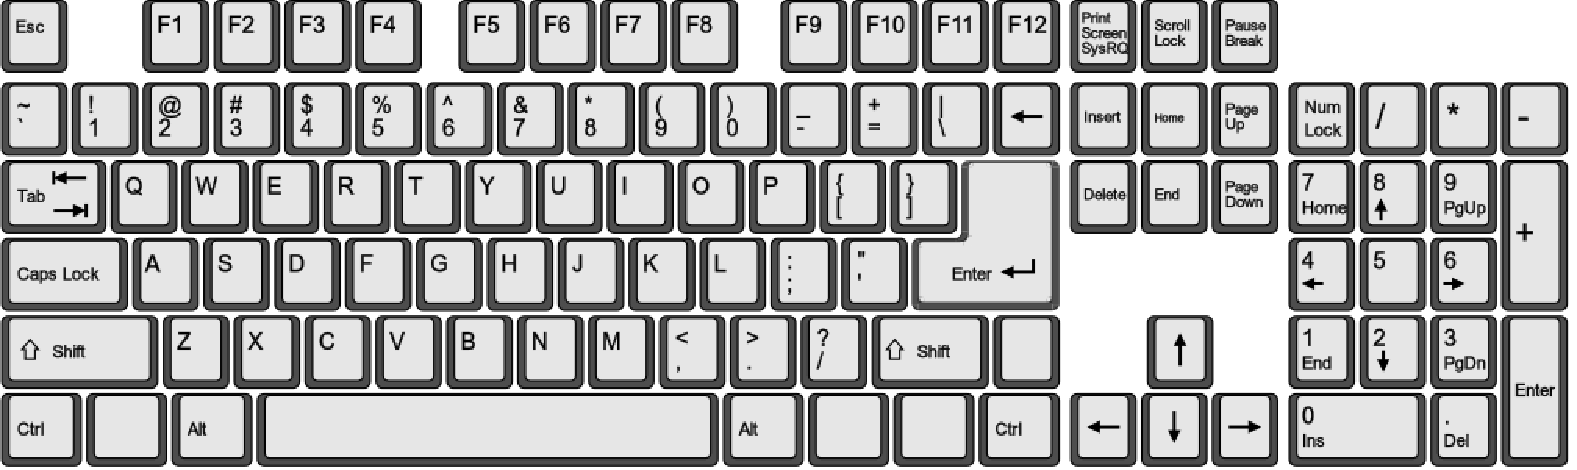
\includegraphics[scale=0.7]{keyboard.pdf} %\centerline{\getpic{keyboard}}
    \caption{This diagram has been produced as svg with dpic -v 
      (then converted to pdf for inclusion in examples.pdf)
    \src{keyboard.m4}.}
  }\fi\fi

\bfig{
    \centerline{\getpic{Dini}}
    \caption{Dini surface and an icosahedron
    \src{Dini.m4}.}
  }

\bfig{
    \centerline{\getpic{Sierpinski}}
    \caption{The Sierpinski triangle and a Cayley graph:
    tests of pic macro recursion
    \src{Sierpinski.m4}.}
  }

\bfig{
    \centerline{\getpic{Escher}}
    \caption{Penrose stairs and an Escher-like object
    \src{Escher.m4}.}
  }

\bfig{
    \centerline{\getpic{recycle}}
    \caption{Modest repetition and partial fill
    \src{recycle.m4}.}
  }

\bfig{
    \centerline{\getpic{ex15}}
    \caption{Simple diagrams that are easily drawn by looping
    \src{ex15.m4}.}
   }

\bfig{
    \centerline{\getpic{Crow}}
    \caption{Illustrating {\tt shadebox} and a custom crowfoot line termination
    \src{Crow.m4}.}
  }

\bfig{
    \centerline{\getpic{Flow}}
    \caption{A flowchart sampler
    \src{Flow.m4}.}
  }

\bfig{
    \centerline{\getpic{Btree}}
    \caption{Trees
    \src{Btree.m4}.}
  }

\ifmpost\else% Tex capacity exceeded at this point under metapost
% Overlaying a figure with line graphics depends on the postprocessor:
\ifpst%                          PSTricks
\bfig{%
    \centerline{\getpic{Incleps}}%
    \caption{Overlaying a figure with line graphics
    \src{Incleps.m4}.}%
  }
\else\ifpgf%                     PGF
\bfig{%
    \centerline{\getpic{Incleps}}% %ignore%
    \caption{Overlaying a figure with line graphics %ignore%
    \src{Incleps.m4}.}%
  }
\else\ifmpost%                   MetaPost
\bfig{%
    \centerline{\boxdims{InclA}{%ignore%
        \includegraphics[width=3in]{../Incl.eps.gz}}%
        \hspace*{-3in}\includegraphics{Inclpdf.1}}%
    \caption{Overlaying a figure with line graphics %ignore%
    \src{Inclpdf.m4}.}
  }
\else\ifpdfl%                    pdflatex
\bfig{%
    \centerline{\boxdims{InclA}{%ignore%
        \includegraphics[width=3in]{../Incl}}%
        \hspace*{-3in}\includegraphics{Incleps}}%
    \caption{Overlaying a figure with line graphics %ignore%
    \src{Incleps.m4}.}
  }
\else\ifpostscript%              Postscript with psfrag (.eps.gz not allowed)
ifpostscript(,\bfig{%
    \centerline{\boxdims{InclA}{%ignore%
        \includegraphics[width=3in]{Incl.eps}}%
        \hspace*{-3in}\includegraphics{Incleps.eps}}%
    \caption{Overlaying a figure with line graphics %ignore%
    \src{Incleps.m4}.}
  })
\fi\fi\fi\fi\fi
\fi % ifmpost

\end{document}
